%%%%%%%% ICML 2020 EXAMPLE LATEX SUBMISSION FILE %%%%%%%%%%%%%%%%%

\documentclass{article}

% Recommended, but optional, packages for figures and better typesetting:
\usepackage{microtype}
\usepackage{graphicx}
\usepackage{subfigure}
\usepackage{booktabs} % for professional tables

% hyperref makes hyperlinks in the resulting PDF.
% If your build breaks (sometimes temporarily if a hyperlink spans a page)
% please comment out the following usepackage line and replace
% \usepackage{icml2020} with \usepackage[nohyperref]{icml2020} above.
\usepackage{hyperref}

% Attempt to make hyperref and algorithmic work together better:
\newcommand{\theHalgorithm}{\arabic{algorithm}}

% Use the following line for the initial blind version submitted for review:
\usepackage{icml2020}

% If accepted, instead use the following line for the camera-ready submission:
%\usepackage[accepted]{icml2020}

% The \icmltitle you define below is probably too long as a header.
% Therefore, a short form for the running title is supplied here:
%\icmltitlerunning{Submission and Formatting Instructions for ICML 2020}


% Custom packages
\usepackage{amsthm}
\usepackage{amsmath}
\usepackage{amssymb}
\usepackage{float}
\usepackage{hyperref}
\usepackage{blkarray}
\usepackage{todonotes}
\usepackage{mathtools}




%%%%%%%%%%%%%%%%%%%%%%%%%%%%
% Paper dependent stuff    %
%%%%%%%%%%%%%%%%%%%%%%%%%%%%

\newcommand{\Tau}{\mathcal{T}}

%%%%%%%%%%%%%%%%%%%%%%%%%%%%
% Aesthetics               %
% over-underline, hat, bold%
%%%%%%%%%%%%%%%%%%%%%%%%%%%%

\newcommand{\eps}{\varepsilon}
\newcommand{\vareps}{\varepsilon}
\renewcommand{\epsilon}{\varepsilon}
%\renewcommand{\hat}{\widehat}
\renewcommand{\tilde}{\widetilde}
\renewcommand{\bar}{\overline}

\newcommand*{\MyDef}{\mathrm{\tiny def}}
\newcommand*{\eqdefU}{\ensuremath{\mathop{\overset{\MyDef}{=}}}}% Unscaled version
% \newcommand*{\eqdef}{\mathop{\overset{\MyDef}{\resizebox{\widthof{\eqdefU}}{\heightof{=}}{=}}}}
\newcommand{\eqdef}{\stackrel{def}{=}}


\def\:#1{\protect \ifmmode {\mathbf{#1}} \else {\textbf{#1}} \fi}
\newcommand{\CommaBin}{\mathbin{\raisebox{0.5ex}{,}}}

\newcommand{\wt}[1]{\widetilde{#1}}
\newcommand{\wh}[1]{\widehat{#1}}
\newcommand{\wo}[1]{\overline{#1}}
\newcommand{\wb}[1]{\overline{#1}}

% bf and bm missing due to conflict!!
\newcommand{\bsym}[1]{\mathbf{#1}}
\newcommand{\bzero}{\mathbf{0}}
\newcommand{\ba}{\mathbf{a}}
\newcommand{\bb}{\mathbf{b}}
\newcommand{\bc}{\mathbf{c}}
\newcommand{\bd}{\mathbf{d}}
\newcommand{\be}{\mathbf{e}}
\newcommand{\bg}{\mathbf{g}}
\newcommand{\bh}{\mathbf{h}}
\newcommand{\bi}{\mathbf{i}}
\newcommand{\bj}{\mathbf{j}}
\newcommand{\bk}{\mathbf{k}}
\newcommand{\bl}{\mathbf{l}}
\newcommand{\bn}{\mathbf{n}}
\newcommand{\bo}{\mathbf{o}}
\newcommand{\bp}{\mathbf{p}}
\newcommand{\bq}{\mathbf{q}}
\newcommand{\br}{\mathbf{r}}
\newcommand{\bs}{\mathbf{s}}
\newcommand{\bt}{\mathbf{t}}
\newcommand{\bu}{\mathbf{u}}
\newcommand{\bv}{\mathbf{v}}
\newcommand{\bw}{\mathbf{w}}
\newcommand{\bx}{\mathbf{x}}
\newcommand{\by}{\mathbf{y}}
\newcommand{\bz}{\mathbf{z}}

\newcommand{\bA}{\mathbf{A}}
\newcommand{\bB}{\mathbf{B}}
\newcommand{\bC}{\mathbf{C}}
\newcommand{\bD}{\mathbf{D}}
\newcommand{\bE}{\mathbf{E}}
\newcommand{\bF}{\mathbf{F}}
\newcommand{\bG}{\mathbf{G}}
\newcommand{\bH}{\mathbf{H}}
\newcommand{\bI}{\mathbf{I}}
\newcommand{\bJ}{\mathbf{J}}
\newcommand{\bK}{\mathbf{K}}
\newcommand{\bL}{\mathbf{L}}
\newcommand{\bM}{\mathbf{M}}
\newcommand{\bN}{\mathbf{N}}
\newcommand{\bO}{\mathbf{O}}
\newcommand{\bP}{\mathbf{P}}
\newcommand{\bQ}{\mathbf{Q}}
\newcommand{\bR}{\mathbf{R}}
\newcommand{\bS}{\mathbf{S}}
\newcommand{\bT}{\mathbf{T}}
\newcommand{\bU}{\mathbf{U}}
\newcommand{\bV}{\mathbf{V}}
\newcommand{\bW}{\mathbf{W}}
\newcommand{\bX}{\mathbf{X}}
\newcommand{\bY}{\mathbf{Y}}
\newcommand{\bZ}{\mathbf{Z}}

% calligraphic
\newcommand{\cf}{\mathcal{f}}
\newcommand{\cA}{\mathcal{A}}
\newcommand{\cB}{\mathcal{B}}
\newcommand{\cC}{\mathcal{C}}
\newcommand{\cD}{\mathcal{D}}
\newcommand{\cE}{\mathcal{E}}
\newcommand{\cF}{\mathcal{F}}
\newcommand{\cG}{\mathcal{G}}
\newcommand{\cH}{\mathcal{H}}
\newcommand{\cI}{\mathcal{I}}
\newcommand{\cJ}{\mathcal{J}}
\newcommand{\cK}{\mathcal{K}}
\newcommand{\cL}{\mathcal{L}}
\newcommand{\cM}{\mathcal{M}}
\newcommand{\cN}{\mathcal{N}}
\newcommand{\cO}{\mathcal{O}}
\newcommand{\cP}{\mathcal{P}}
\newcommand{\cQ}{\mathcal{Q}}
\newcommand{\cR}{\mathcal{R}}
\newcommand{\cS}{\mathcal{S}}
\newcommand{\cT}{\mathcal{T}}
\newcommand{\cU}{\mathcal{U}}
\newcommand{\cV}{\mathcal{V}}
\newcommand{\cW}{\mathcal{W}}
\newcommand{\cX}{\mathcal{X}}
\newcommand{\cY}{\mathcal{Y}}
\newcommand{\cZ}{\mathcal{Z}}

%%%%%%%%%%%%%%%%%%%%%%%%%%%%
% Math jargon              %
%%%%%%%%%%%%%%%%%%%%%%%%%%%%
\newcommand{\wrt}{w.r.t.\xspace}
\newcommand{\defeq}{\stackrel{\mathclap{\normalfont\mbox{\tiny def}}}{=}}
\newcommand{\maxund}[1]{\max\limits_{#1}}
\newcommand{\supund}[1]{\text{sup}\limits_{#1}}
\newcommand{\minund}[1]{\min\limits_{#1}}
\renewcommand{\epsilon}{\varepsilon}
\newcommand{\bigotime}{\mathcal{O}}


\DeclareMathOperator*{\argmin}{arg\,min} 
\DeclareMathOperator*{\argmax}{arg\,max} 
\DeclareMathOperator*{\cupdot}{\mathbin{\mathaccent\cdot\cup}}

%%%%%%%%%%%%%%%%%%%%%%%%%%%%
% Matrix operators         %
%%%%%%%%%%%%%%%%%%%%%%%%%%%%
\newcommand{\transpose}{^\mathsf{\scriptscriptstyle T}}
\newcommand{\transp}{\mathsf{\scriptscriptstyle T}}
\DeclareMathOperator{\Tr}{Tr}
\DeclarePairedDelimiterX{\inp}[2]{\langle}{\rangle}{#1, #2}

%%%%%%%%%%%%%%%%%%%%%%%%%%%%
% Statistic operators      %
%%%%%%%%%%%%%%%%%%%%%%%%%%%%
\newcommand{\probability}[1]{\mathbb{P}\left(#1\right)}
\newcommand{\probdist}{Pr}
\DeclareMathOperator*{\expectedvalue}{\mathbb{E}}
\DeclareMathOperator*{\variance}{\text{Var}}
\newcommand{\expectedvalueover}[1]{\expectedvalue\limits_{#1}}
\newcommand{\condbar}{\;\middle|\;}
\newcommand{\gaussdistr}{\mathcal{N}}
\newcommand{\uniformdistr}{\mathcal{U}}
\newcommand{\bernoullidist}{\mathcal{B}}

%%%%%%%%%%%%%%%%%%%%%%%%%%%%
% Algebraic Sets           %
%%%%%%%%%%%%%%%%%%%%%%%%%%%%
\newcommand{\Real}{\mathbb{R}}
\newcommand{\Natural}{\mathbb{N}}
\newcommand{\statespace}{\mathcal{X}}
\newcommand{\funcspace}{\mathcal{F}}
\newcommand{\dynaspace}{\mathcal{T}}


\newtheorem{theorem}{Theorem}
\newtheorem{definition}{Definition}
\newtheorem{lemma}{Lemma}
\newtheorem{proposition}{Proposition}
\providecommand*\propositionautorefname{Proposition}
\newtheorem{remark}{Remark}
\newtheorem{property}{Property}
\newtheorem{assumption}{Assumption}
\providecommand*\assumptionautorefname{Assumption}
\newtheorem{conjecture}{Conjecture}

\newtheorem*{definition*}{Definition}
\newtheorem*{theorem*}{Theorem}
\newtheorem*{proposition*}{Proposition}
\newtheorem*{remark*}{Remark}
\newtheorem*{example*}{Example}

%\author{Edouard Leurent, Denis Efimov, Odalric-Ambrym Maillard}



\begin{document}
	
	\twocolumn[
	\icmltitle{Robust Estimation, Prediction and Control with \\ Continuous States and Dynamics Structure}
	
	% It is OKAY to include author information, even for blind
	% submissions: the style file will automatically remove it for you
	% unless you've provided the [accepted] option to the icml2020
	% package.
	
	% List of affiliations: The first argument should be a (short)
	% identifier you will use later to specify author affiliations
	% Academic affiliations should list Department, University, City, Region, Country
	% Industry affiliations should list Company, City, Region, Country
	
	% You can specify symbols, otherwise they are numbered in order.
	% Ideally, you should not use this facility. Affiliations will be numbered
	% in order of appearance and this is the preferred way.
	\icmlsetsymbol{equal}{*}
	
	\begin{icmlauthorlist}
		\icmlauthor{Edouard Leurent}{seq,val,ren}
		\icmlauthor{Denis Efimov}{val}
		\icmlauthor{Odalric Ambrym-Maillard}{seq}
	\end{icmlauthorlist}
	
	\icmlaffiliation{seq}{Inria Lille Nord-Europe, Sequel Project, Lille, France}
	\icmlaffiliation{val}{Inria Lille Nord-Europe, Valse Project, Lille, France}
	\icmlaffiliation{ren}{Renault Group, Guyancourt, France}
	
	\icmlcorrespondingauthor{Edouard Leurent}{edouard.leurent@inria.fr}
	
	% You may provide any keywords that you
	% find helpful for describing your paper; these are used to populate
	% the "keywords" metadata in the PDF but will not be shown in the document
	\icmlkeywords{Machine Learning, ICML}
	
	\vskip 0.3in
	]
	
	% this must go after the closing bracket ] following \twocolumn[ ...
	
	% This command actually creates the footnote in the first column
	% listing the affiliations and the copyright notice.
	% The command takes one argument, which is text to display at the start of the footnote.
	% The \icmlEqualContribution command is standard text for equal contribution.
	% Remove it (just {}) if you do not need this facility.
	
	\printAffiliationsAndNotice{}  % leave blank if no need to mention equal contribution
%	\printAffiliationsAndNotice{\icmlEqualContribution} % otherwise use the standard text.
	
	\begin{abstract}
		This document provides a basic paper template and submission guidelines.
		Abstracts must be a single paragraph, ideally between 4--6 sentences long.
		Gross violations will trigger corrections at the camera-ready phase.
	\end{abstract}

\section{Introduction}

\section{Related Work}

For LQ systems, where parameters A,B are unknown and no structure is available.
\begin{itemize}
    \item OFU: \citep{abbasi-yadkori11a}. Summary: $\theta=(A~B)$, ellipsoid in Frobenius norm + controllability constraint, choose and stabilize (Ricatti) an optimistic candidate, cumulative regret in $O(\sqrt{T}\log\frac{1}{\delta})$.
    \item PSRL with TS: \citep{abeille18a}. Summary: RLS estimate + normal perturbation in the ellipsoid + rejection sampling over a controllability constraint, with frequent update, cumulative regret in $\tilde{O}(\sqrt{T})$
    \item Offline estimation and control synthesis: \citep{Dean2017}. Summary: Estimation procedure of $N$ episodes of duration $T$ with gaussian excitation, ellipsoid in L2 norm, robust controller with System Level Synthesis, simple regret in $O(\sqrt{\frac{\log(1/\delta)}{N}})$
    \item \citep{Dean2018}
\end{itemize}

Differences with our work:
\begin{itemize}
    \item We wish to act straight away in a reasonable (structure) but cautious (robust) way, and progressively get more and more aggressive as we obtain more data and reduce uncertainty.
    \item Thus, we do not wish to explore actively the more promising regions as in OFU, nor the more likely region as in TS, nor act randomly as in Coarse-ID.
    \item We have linear dynamics but our cost is not quadratic. Thus, we can accurately represent planning tasks with discrete/branching decisions involving discontinuities (e.g. collision vs non-collision states).
    \item Our optimisation problem amounts to a sequence of controllers selection, instead of continuous controller synthesis
    
\end{itemize}

\section{Problem formulation}

\paragraph{Structured dynamics}
We consider a system with dynamics in the form:

\begin{equation}
\label{eq:dynamics}
\dot{x}(t)=A(\theta)x(t) + B u(t) + D \omega(t),\;t\geq0,
\end{equation}
with state $x\in\Real^p$, control $u\in\Real^q$, and disturbance $\omega\in\Real^s$. The dynamics $A(\theta)\in\Real^{p\times p}$  is parametrised by $\theta$ that belongs to a compact set $\Theta \subset \Real^d$. The control matrix $B\in\Real^{p\times q}$ and disturbance matrix $D\in\Real^{p\times s}$ are known.

We also have access to a measurement of the form
$
    \dot{x}(t) + C\nu(t)
$
that we will actually denote (since the control $u(t)$ is known) as:
\begin{equation}
\label{eq:measurement}
    y(t) = \dot{x}(t) - Bu(t) + C\nu(t)
\end{equation}
where $\nu(t)\in\Real^r$ is a measurement noise and $C\in\Real^{p\times r}$ is known. Assumptions over the disturbance $\omega$ and noise $\nu$ will be detailed further.

\paragraph{Objective}

We wish to find a sequence of commands $\pi=(u_t)_{t\geq 0}$ that maximises a cumulative objective $V^\pi$:
\todo[inline]{EL: since the interval dynamics will be deterministic, use open-loop policies, ie sequences of actions $\mathbf{u}$ instead of closed-loop policies $\pi$}

\todo[inline]{EL: the prediction is done in continuous time and the control in discrete time. How to handle the change in notations?}

\begin{equation}
\max_\pi V^\pi
\end{equation}
where
\begin{equation}
\label{eq:optimal-control}
V^\pi = \expectedvalueover{\omega(t)}\left[\sum_{t=0}^\infty \gamma^t r(x(t))\condbar u_t = \pi(x_t),\,\eqref{eq:dynamics}\right]
\end{equation}
and $r:\Real^p\rightarrow[0,1]$ is a bounded reward function.

\section{Model Estimation}

\paragraph{Objective}
Having observed at times $(t_n)_{n\in[N]}$ a history of transitions $\cD = \{(x_n = x(t_n), u_n = u(t_n), y_n = y(t_n))\}_{n\in[N]}$, and given a confidence level $\delta\in[0, 1]$, our goal is to find a confidence region $\cC_\delta$ as tight as possible and such that it holds that:
\begin{align}
\probability{A(\theta)\in \cC_\delta} \geq 1-\delta
\label{eq:polytope}
\end{align}

% This involves the trilemma of confidence intervals, where one of three things must be true:
% \begin{enumerate}
%     \item $A(\theta)$ is in $\cC_\delta$
%     \item We got data that was very ($\leq\delta$) unlikely under all possible values $A(\theta)$
%     \item Our model is wrong
% \end{enumerate}

% \paragraph{Tensor notations}
% We adopt the notations of [Tensor Decompositions and Applications]:
% Given a tensor $A\in\Real^{I_1\times\cdots\times I_l}$ and matrix $M\in\Real^{I_n\times J}$, the $n$-mode product of $A$ by $M$ is a tensor of $\Real^{I_1\times\cdots\times I_l}$  defined by:
% \begin{equation*}
%     (A\times_n M)_{i_1,\cdots,i_{n-1},j,i_{n+1},\cdots,i_l} = \sum_{k=1}^{I_n} A_{i_1,\cdots,i_{n-1},k,i_{n+1},\cdots,i_l}B_{k,j}
% \end{equation*}

We further assume that the dynamics $A(\theta)$ enjoy the following additional structure:
\begin{assumption}[Linear parametrisation]
\label{assumpt:linear_param}
There exists a known tensor $\phi\in \Real^{d \times p \times p}$ such that for all $\theta\in\Theta$:
\begin{equation}
    A(\theta) = \theta^\transp \phi \eqdef \sum_{i=1}^d \theta_i\phi_i
\end{equation}
where $\phi_i\in\Real^{p\times p}$ for all $i\in[d]$.

For all $n\geq 0$, we also denote $\Phi_n = [\phi_1 x_n \cdots \phi_d x_n]\in\Real^{p\times d}$.
\end{assumption}


\paragraph{Regularised least square} Since we expect that $\Phi_n$ may have zero-coordinates during possibly long time intervals (i.e. some features are not always active), we consider the weighted $L_2$-regularised regression problem with weights  $\Sigma_p\in\Real^{p\times p}$ and $\Sigma_d\in\Real^{d\times d}$ and parameter $\lambda\in\Real^+_*$:


\begin{equation}
    \label{eq:regression_min}
    \min_{\theta\in\Real^d} \sum_{n=1}^N \|y_n -\Phi_n\theta\|_{\Sigma_p^{-1}}^2 + \lambda\|\theta\|_{\Sigma_d}^2
\end{equation}


The solution can be obtained as:

\begin{theorem}[Regularised solution]
\label{thm:regularized_solution}
The solution to \eqref{eq:regression_min} is:
\begin{equation}
    \label{eq:vector_rls}
    \theta_{N,\lambda} = G_{N, \lambda}^{-1} \sum_{n=1}^N \Phi_n^\transp \Sigma_p^{-1} y_n
\end{equation}
where 
\begin{equation*}
    G_{N, \lambda} = \sum_{n=1}^N \Phi_{n}^\transp\Sigma_p^{-1}\Phi_{n}  + \lambda \Sigma_d \in \Real^{d\times d}.
\end{equation*}
\end{theorem}

Denote $\eta(t) = C\nu(t) + D\omega(t)$. By substituting the expression of $y_n$ into \eqref{eq:vector_rls}, we obtain:
\begin{lemma}[Regression error]
\label{lem:regression-error}
\begin{align*}
    \theta_{N,\lambda} - \theta = G_{N, \lambda}^{-1}\sum_{n=1}^N \Phi_n^\transp \Sigma_p^{-1}\eta_n - G_{N, \lambda}^{-1}\lambda\Sigma_d\theta 
\end{align*}
\end{lemma}

Depending on the assumption we take over the noise $\eta_n$ and the true parameter $\theta$, we can bound the regression error $\theta_{N,\lambda} - \theta$ in different ways.

\subsection{Sub-Gaussian noise}

We say that a random vector $x\in\Real^k$ is sub-Gaussian with covariance proxy $\Sigma$, and denote $x\sim Sub_G(\Sigma)$, if $\expectedvalue[x] = 0_k$ and:
\[
\forall u\in\Real^k, \expectedvalue \left[ \exp{\left( u^\transp x\right)}\right] \leq \exp{\left( \frac{1}{2} u^\transp \Sigma u\right)}
\]

\begin{assumption}[Sub-Gaussian Noise Model]
\label{assumpt:noise}
At each time $t\geq0$ the sum $\eta(t)$ of projected measurement noise $\nu(t)$ and disturbance $\omega(t)$ is a Sub-Gaussian noises with covariance proxy $\Sigma_p \in \Real^{p\times p}$:
\begin{equation*}
    \eta(t) = C\nu(t) + D\omega(t) \sim Sub_G(\Sigma_p)
\end{equation*}

For instance, this is the case of $\nu$ and $\omega$ are Gaussian noises with respective covariance matrices $\Sigma_r$ and $\Sigma_s$, with $\Sigma_p \eqdef C\Sigma_r C^\transp + D\Sigma_s D^\transp$.
\end{assumption}

\begin{lemma}[Theorem 1 of \citep{Abbasi2011}, Matrix version]
\label{lem:concentration}
Let $\{F_t\}_{t=0}$ be a filtration.
Let $\{\eta_t\}_{t=1}^\infty$ be a $\Real^p$-valued stochastic process such that $\eta_t$ is $F_t$-measurable and conditionally $\Sigma_p$-SubGaussian.

Let $\{\Phi_t\}_{t=1}^\infty$ be an $\Real^{p\times d}$-valued stochastic process such that $\Phi_t$ is $F_t$-measurable. Assume that $G$ is a $d\times d$ positive definite matrix. For any $t\geq 0$, define:

\begin{equation*}
    \overline{G}_t = G + \sum_{s=1}^t \Phi_s^\transp \Sigma_p^{-1} \Phi_s \in \Real^{d\times d} \qquad S_t = \sum_{s=1}^t \Phi_s^\transp\Sigma_p^{-1}\eta_s \in \Real^{d}
\end{equation*}
Then, for any $\delta>0$, with probability at least $1-\delta$, for all $t\geq0$

\begin{align*}
    \|S_t\|_{\overline{G_t}} \leq \cdots
\end{align*}
\end{lemma}

\begin{theorem}[Confidence ellipsoid]
\label{thm:confidence_ellipsoid}
\todo[inline]{TODO}
\end{theorem}

\begin{lemma}[Confidence polytope]
\label{lem:confidence_polytope}
We can enclose the confidence ellipsoid $C_\delta$ obtained in $\eqref{eq:confidence-ellipsoid}$ within a polytope $P_\delta$:
\[\cC_\delta \subset \cP_\delta\]
where $\cP_\delta$ can be written as:
\begin{equation}
     \cP_\delta = \left\{ A_{0}+\sum_{i=1}^{2^d}\lambda_{i}\Delta A_{i}: \lambda\in[0, 1]^{2^d},  \sum_{i=1}^{2^d}\lambda_{i}=1\right\}.
\end{equation}
with 
\begin{align*}
    &G_{N,\lambda}^{-1} = PDP^{-1}\\
    &h_k \text{ is the }k^\text{th}\text{ element of }\{-1,1\}^d\text{, for } k\in[2^d]\\
    &\Delta\theta_k = C_{N,\lambda,\delta}^{1/2} P^{-1}D^{-1/2} h_k \\
    &A_0 = \theta_{N,\lambda}^\transp\Phi\\
    &\Delta A_k = \Delta\theta_k^\transp\Phi\\
\end{align*}
This conversion is illustrated in \autoref{fig:ellipsoid_to_polytope}
\end{lemma}

\begin{figure}
    \centering
    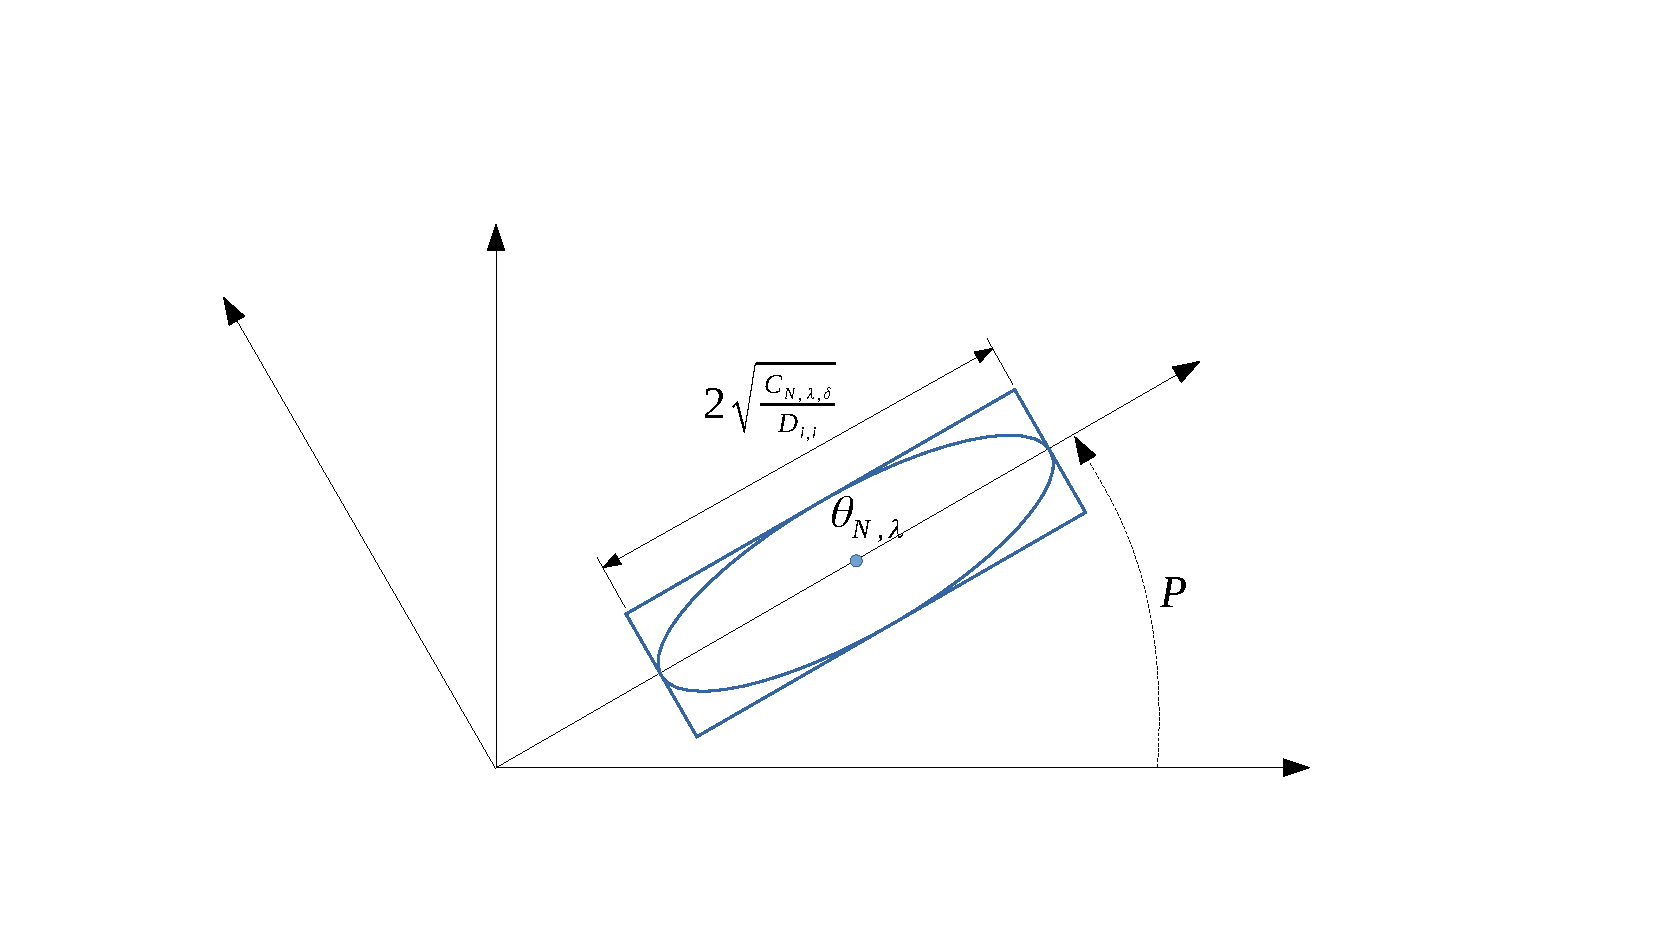
\includegraphics[trim={3.8cm, 2cm, 5cm, 3.8cm}, clip, width=0.4\textwidth]{img/ellipsoid_to_polytope}
    \caption{From the confidence ellipsoid $\cC_\delta$ to its enclosing polytope $\cP_\delta$}
    \label{fig:ellipsoid_to_polytope}
\end{figure}

\subsection{Bounded noise}

\begin{assumption}[Bounded noise]
The noise $\eta(t) = C\nu(t) + D\omega(t)$ is bounded.
\[\|\eta\|_\infty < \infty\]
\end{assumption}

Then, 
\begin{align*}
\|\theta_{N,\lambda} - \theta\|_1 &\leq \|G_{N, \lambda}^{-1}\sum_{n=1}^N \Phi_n^\transp \Sigma_p^{-1}\|_1\|\eta\|_\infty + \lambda\|G_{N, \lambda}^{-1}\Sigma_d\theta\|_1\\
&\leq \|G_{N, \lambda}^{-1}\sum_{n=1}^N \Phi_n^\transp \Sigma_p^{-1}\|_1\|\eta\|_\infty + \lambda\|G_{N, \lambda}^{-1}\Sigma_d\|_1\|\theta\|_\infty
\end{align*}


This $L_1$-ball is a polytope with $2d$ vertices, that we denote $\cP$.

\section{State Prediction}

In this section, we assume that we found a high-confidence polytope that verifies \eqref{eq:polytope} with probability $1-\delta$.

The objective of the prediction procedure, as illustrated in \autoref{fig:interval-hull} is to design an \emph{interval predictor} for the system \eqref{eq:dynamics}, which takes the information on the observed current state ${x}({0})$, the admissible bounds on the perturbation $[\underline{\omega}(t),\overline{\omega}(t)]$, and the model polytope $\cP_\delta$, and verifies the inclusion property:
\begin{equation}
\label{eq:interval_property}
\underline{x}(t)\leq x(t)\leq\overline{x}(t),\quad\forall t\geq0.
\end{equation}

\begin{figure}
    \centering
    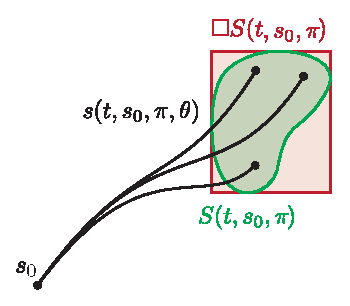
\includegraphics[width=0.3\textwidth]{img/interval-hull}
    \caption{A few trajectories are sampled from an initial state $x_0$ following a policy $\pi=(u_0,\cdots)$ with various parameters $\theta$ (in black). The union of reachability sets is shown in green, and its interval hull in red.}
    \label{fig:interval-hull}
\end{figure}

In order to use the interval predictor from \citep{leurent2019interval}, we also require $A_0$ to be Metzler. This can be ensured under some conditions:

\begin{lemma}[Similarity transformation \citep{Efimov_a2013}]
\label{lem:metzler} Let $D\in\Xi\subset\Real^{n\times n}$ be a matrix variable satisfying the interval constraints $\Xi=\{D\in\Real^{n\times n}:\,D_{a}-\Delta\le D\le D_{a}+\Delta\}$ for some $D_{a}^{\text{T}}=D_{a}\in\Real^{n\times n}$ and $\Delta\in\Real_{+}^{n\times n}$. If for some constant $\mu\in\Real_{+}$ and a diagonal matrix $\Upsilon\in\Real^{n\times n}$ the Metzler matrix $Y=\mu E_{n\times n}-\Upsilon$ has the same eigenvalues as the matrix $D_{a}$, then there is an orthogonal matrix $S\in\Real^{n\times n}$ such that the matrices $S^{\text{T}}DS$ are Metzler for all $D\in\Xi$ provided that $\mu>n||\Delta||_{max}$.\textup{ }
\end{lemma}

\begin{theorem}[Interval Predictor \citep{leurent2019interval}]
\label{thm:predictor}
Assuming that \eqref{eq:polytope} is satisfied for the system \eqref{eq:dynamics}, then the interval predictor:
\begin{eqnarray}
\dot{\underline{x}}(t) & = & A_{0}\underline{x}(t)-\Delta A_{+}\underline{x}^{-}(t)-\Delta A_{-}\overline{x}^{+}(t)\nonumber \\
 &  & +Bu(t)+D^{+}\underline{\omega}(t)-D^{-}\overline{\omega}(t),\nonumber\\
\dot{\overline{x}}(t) & = & A_{0}\overline{x}(t)+\Delta A_{+}\overline{x}^{+}(t)+\Delta A_{-}\underline{x}^{-}(t) \label{eq:interval_predictor} \\
 &  & +Bu(t)+D^{+}\overline{\omega}(t)-D^{-}\underline{\omega}(t),\nonumber \\
 &  & \underline{x}(0)=\underline{x}_{0},\;\overline{x}(0)=\overline{x}_{0}\nonumber 
\end{eqnarray}
ensures the inclusion property \eqref{eq:interval_property}. If there exist diagonal matrices $P$, $Q$, $Q_{+}$, $Q_{-}$, $Z_{+}$, $Z_{-}$, $\Psi_{+}$, $\Psi_{-}$, $\Psi$, $\Gamma\in\Real^{2n\times 2n}$ such that the following LMIs are satisfied:
\begin{gather*}
P+\min\{Z_{+},Z_{-}\}>0,\;\Upsilon\preceq0,\;\Gamma>0,\\
Q+\min\{Q_{+},Q_{-}\}+2\min\{\Psi_{+},\Psi_{-}\}>0,
\end{gather*}
where{\footnotesize{}
\begin{gather*}
\Upsilon=\left[\begin{array}{cccc}
\Upsilon_{11} & \Upsilon_{12} & \Upsilon_{13} & P\\
\Upsilon_{12}^{\top} & \Upsilon_{22} & \Upsilon_{23} & Z_{+}\\
\Upsilon_{13}^{\top} & \Upsilon_{23}^{\top} & \Upsilon_{33} & Z_{-}\\
P & Z_{+} & Z_{-} & -\Gamma
\end{array}\right],\\
\Upsilon_{11}=\mathcal{A}^{\top}P+P\mathcal{A}+Q,\;\Upsilon_{12}=\mathcal{A}^{\top}Z_{+}+PR_{+}+\Psi_{+},\\
\Upsilon_{13}=\mathcal{A}^{\top}Z_{-}+PR_{-}+\Psi_{-},\;\Upsilon_{22}=Z_{+}R_{+}+R_{+}^{\top}Z_{+}+Q_{+},\\
\Upsilon_{23}=Z_{+}R_{-}+R_{+}^{\top}Z_{-}+\Psi,\;\Upsilon_{33}=Z_{-}R_{-}+R_{-}^{\top}Z_{-}+Q_{-},\\
\mathcal{A}=\left[\begin{array}{cc}
A_{0} & 0\\
0 & A_{0}
\end{array}\right],\;R_{+}=\left[\begin{array}{cc}
0 & -\Delta A_{-}\\
0 & \Delta A_{+}
\end{array}\right],\;R_{-}=\left[\begin{array}{cc}
\Delta A_{+} & 0\\
-\Delta A_{-} & 0
\end{array}\right],
\end{gather*}
}then the predictor \eqref{eq:interval_predictor} is input-to-state stable with respect to the inputs $\underline{\omega}$, $\overline{\omega}$.
\end{theorem}

% \begin{example*}
% Consider a scalar system:
% \[
% \dot{x}(t)=-\theta(t)x(t)+d(t),\;t\geq0,
% \]
% where $x(t)\in\Real$ with $x(0)\in[\underline{x}_{0},\overline{x}_{0}]=[1.0, 1.1]$, $\theta(t)\in\Pi=[\underline{\theta},\overline{\theta}]=[0.5,1.5]$ and $d(t)\in[\underline{d},\overline{d}]=[-0.1,0.1]$ for all $t\geq0$. The \autoref{fig:predictor_example} shows the state-interval obtained with \eqref{eq:interval_predictor}.

% \begin{figure}
% \begin{centering}
% 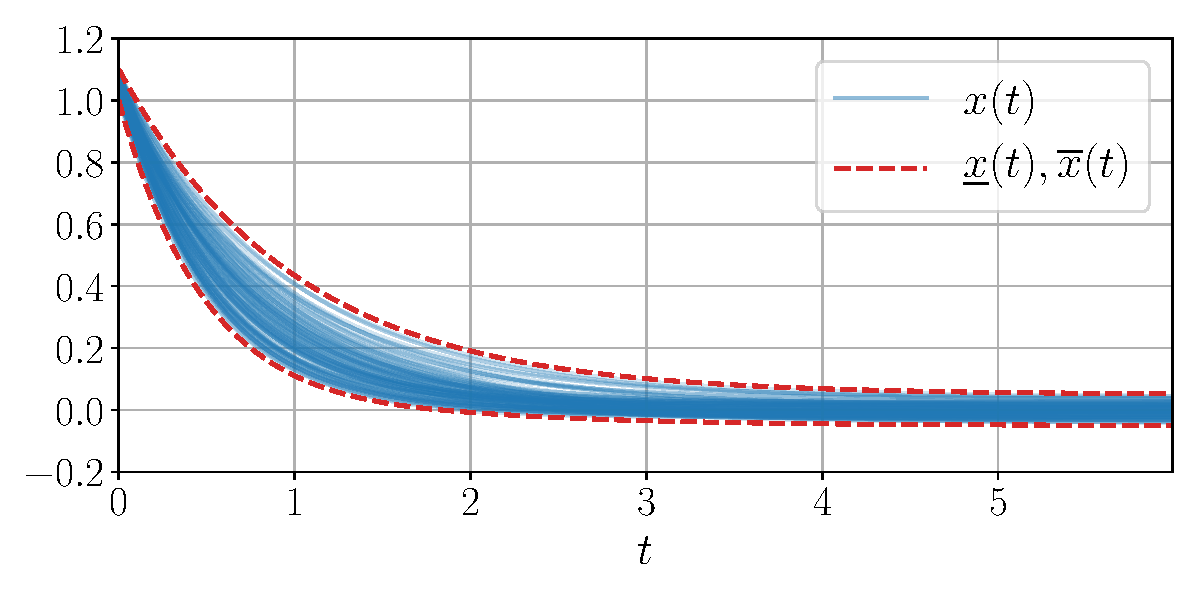
\includegraphics[width=\linewidth]{img/interval_predictor}
% \par\end{centering}
% \caption{Several trajectories for different values of $\theta\in\Theta$ are shown in blue. The result of prediction by \eqref{eq:interval_predictor} is in red: the predictor is stable and produces tight bounds.}
% \label{fig:predictor_example}
% \end{figure}
% \end{example*}

\section{Control}

We consider the robust control objective $v^r$:
\todo[inline]{EL: since the interval dynamics will be deterministic, use open-loop policies, ie sequences of actions $\mathbf{u}$ instead of closed-loop policies $\pi$}

\begin{equation}
\label{eq:robust-control}
\max_\pi \underbrace{\min_{A(\theta) \in \cP} \left[\sum_{t=0}^\infty \gamma^t r(x(t))\condbar u_t = \pi(x_t), \omega(t)\right]}_{v^r(\pi)}
\end{equation}


\begin{definition}[Surrogate objective]
We approximate the robust objective $v^r$ in \eqref{eq:robust-control} by replacing the true reachability set by its interval prediction $[\underline{x}(t), \overline{x}(t)]$ based on the polytopic approximation $\cP_\delta$ of $A(\Theta)$: 

\begin{equation}
\hat{v}^r(\pi) \eqdef \sum_{t=0}^\infty \gamma^t \min_{x\in[\underline{x}(t, \pi), \overline{x}(t, \pi)]}  r(x)
\end{equation}
where $\underline{x}(t, \pi), \overline{x}(t, \pi)$ follow the dynamics defined in \eqref{eq:interval_predictor}.
\end{definition}

%\begin{algorithm}[tp]
%  \SetAlgoLined\DontPrintSemicolon
%  \SetKwFunction{algo}{robust\_control}
%  \SetKwFunction{proc}{pessimistic\_step}
%  \SetKwProg{myalg}{Algorithm}{}{}
%  \myalg{\algo{$s_0$}}{
%  \While{resources available}
%  {
%  Select a candidate action sequence $a$ with a planning algorithm.\;
%  Sample a pessimistic transition and reward $\underline{r}_t$ using \proc{$\underline{x}(t)$, $\overline{x}(t)$, a}.
% \;
% Update the planning algorithm with the sampled pessimistic transition.
%  }
%  \KwRet $\argmax_{\pi\in\Pi} \hat{v^r}(\pi)$ \;}{}
%  \setcounter{AlgoLine}{0}
%  \SetKwProg{myproc}{Procedure}{}{}
%  \myproc{\proc{$\underline{x}(t)$, $\overline{x}(t)$, $a$}}{
%  Integrate \eqref{eq:interval_predictor} over $dt$ with controls $a$ to compute $\underline{x}(t+dt), \overline{x}(t+dt)$\;
%  Compute worst-case reward $\underline{r}_t = \min_{x\in[\underline{x}(t), \overline{x}(t)]} r(x)$\;
%  \KwRet $\underline{x}(t+dt), \overline{x}(t+dt), \underline{r}_t$\;}
%\caption{Interval-based Robust Control}
%\label{algo:irc}
%
%\end{algorithm}

\begin{property}[Lower bound]
\label{prop:lower-bound}
With high probability, the surrogate objective $\hat{v}^r$ is a lower bound of the true objective $v^r$:

\begin{equation}
\hat{v}^r(\pi) \leq v^r(\pi)
\end{equation}

If we assume that $R$ is $L$-Lipschitz, then we can bound the other side:
\begin{equation*}
     \hat{v}^r(\pi) \leq v^r(\pi) \leq \hat{v}^r(\pi) + L\sum_{t=0}^\infty \gamma^t \mu([\underline{x}_N(t),\overline{x}_N(t)])
\end{equation*}
\end{property}


The robust objective error $v^r - \hat{v^r}$ stems from two terms: the approximation of the reachable set by the polytopic and interval approximations and the loss of time-dependency between the states within a single trajectory. If both these approximations are tight enough, maximising the lower bound $\hat{v^r}$ will increase the true objective $v^r$, which is the idea behind Algorithm \ref{algo:irc}.

\section{Multi-model Estimation and Control}

What if our system dynamics \eqref{eq:dynamics} or linear parametrisation assumption \ref{assumpt:linear_param} are wrong?

\subsection{Model adequacy}

We can test the model adequacy, and eventually reject it.

This suggest using multiple models with different sets of features.

\subsection{Robust control with Discrete Ambiguity}


\begin{assumption}[Multi-model ambiguity]
Assume that the true dynamics $f$ lies within a finite set of candidate models $f^1, \cdots, f^M$.
\begin{equation}
\exists m\in[M]: \dot{x}(t) = f^M(x(t), u(t)), \forall t\geq 0
\end{equation}

We temporarily ignore the parametric uncertainty $\theta\in\Theta$ to only consider known deterministic models.
\end{assumption}

\begin{definition}[Robust sequence upper bounds] We define an upper-bound for the value of sequences of actions:
\begin{equation}
\label{eq:robust_sequence_ucb}
b_i^r(n)  \eqdef
\begin{cases}
\min_{m\in[1, M]} \sum_{t=0}^{d-1} \gamma^t r_t^m  + \frac{\gamma^d}{1-\gamma} &\text{if } i \in \mathcal{L}_n \text{ ;}\\
\max_{a\in\mathcal{A}} b_{ia}^r(n) & \text{if } i \in \mathcal{T}_n \setminus \mathcal{L}_n 
\end{cases}
\end{equation}
where $r_t^m$ is the reward obtained at step $t$ by following $i$ with dynamics $f^m$.
\end{definition}
An illustration of the computation of the robust b-values is presented in Figure \ref{fig:drop}.


\begin{figure}
\centering
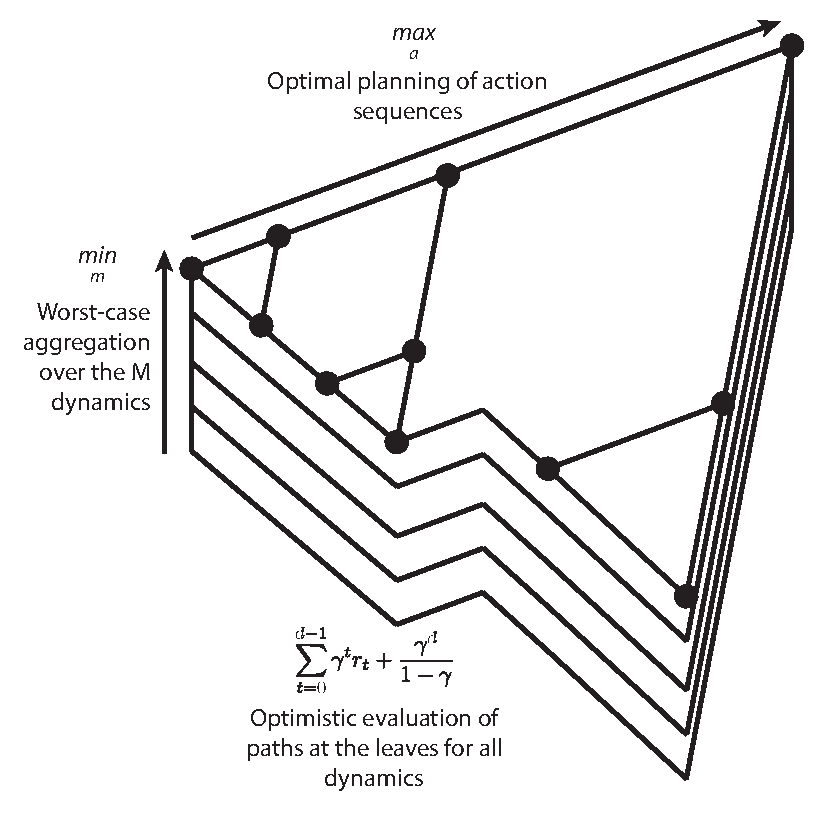
\includegraphics[width=0.3\linewidth]{img/robust-control-tree}
\caption{The computation of robust b-values in Algorithm \ref{algo:drop}. The simulation of trajectories for every dynamics model $f^m$ is represented as stacked versions of the expanded tree $\mathcal{T}_n$.}
\label{fig:drop}
\end{figure}

From this definition we introduce Algorithm \ref{algo:drop}, and analyse its sample-efficiency in Theorem \ref{theorem:drop-regret}.

%\begin{algorithm}[tp]
%\DontPrintSemicolon
%Initialize $\mathcal{T}$ to a root and expand it. Set $n=1$.\;
%\While{Numerical resource available for episode $n$}{
%Compute the robust b-values $b^r_i(n)$.\;
%Expand the leaf $\argmax_{i\in \mathcal{L}_n} b^r_i(n)$.\;
%}
%\Return $\argmax_{a\in \mathcal{A}} u^r_a(n)$
%\caption{Deterministic Robust Optimistic Planning}
%\label{algo:drop}
%\end{algorithm}

The simple regret of the action $a$ returned by Algorithm \ref{algo:drop} after $n$ rounds is defined as:
\begin{equation}
\mathcal{R}_n = v^r - v_a^r
\end{equation}
We will say that $\mathcal{R}_n=O(\varepsilon)$ for some $\varepsilon>0$ if there exist $\rho>0$ and $n_0>0$ such that $\mathcal{R}_n\leq\rho\varepsilon$ for all $n\geq n_0$.
A node $i\in\mathcal{T}$ is said to be $\epsilon$-optimal, in a robust sense, if and only if $v_i^r \geq v^r - \epsilon$ for some $\epsilon > 0$. The proportion of $\epsilon$-optimal nodes at depth $d$ is then defined as $p_d(\epsilon) = |i \in \mathcal{A}^d$ s.t $i$ is $\epsilon$-optimal$|/K^d$. Further we will assume that for the graph $\mathcal{T}$ the following hypothesis is satisfied:
\begin{assumption}[Proportion of near-optimal nodes]
\label{assumpt:beta}
There exist $\beta\in[0, \frac{\log K}{\log 1/\gamma}]$, $c > 0$ and $d_0 > 0$ such that $p_d(\epsilon)\leq c\epsilon^\beta$ for all $\epsilon > 0$ and $d\geq d_0$.
\end{assumption}

\begin{theorem}[Regret bound]
\label{theorem:drop-regret}
Let $\kappa = K\gamma^\beta \in [1, K]$. Then the simple regret of Algorithm \ref{algo:drop} is:


\begin{equation}
\text{If } \kappa>1,\qquad 
\mathcal{R}_n = O\left(n^{-\frac{\log 1/\gamma}{\log \kappa}}\right)
\end{equation}

\begin{equation}
\text{If }\kappa=1,\qquad
\mathcal{R}_n = O\left(\gamma^{\frac{(1-\gamma)^\beta}{c}n}\right)
\end{equation}
\end{theorem}

\section{The Use-Case of Autonomous Driving}


We consider the problem of safe decision-making for autonomous highway driving. An autonomous vehicle is driving on a highway populated with $N$ other agents, and uses Model Predictive Control to plan a sequence of decisions. To that end, it relies on parametrized dynamical model for each agent to predict the future trajectory of each traffic participant: \[\dot{z}_i=f_i(Z,\theta_i),\;i=\overline{1,N},\] where $f_i$ are described below, $z_i\in\Real^4$ is the state of an agent, $Z = [z_1,\dots,z_N]^\top\in\Real^{4N}$ and $\theta_i\in\Real^5$ is the corresponding vector of unknown parameters. Crucially, this system describes the couplings and interactions between vehicles, so that the autonomous agent can properly anticipate their reactions. 
However, we assume that we do not have access to the true values of the behavioural parameters $\theta=[\theta_1,\dots,\theta_N]^\top$; instead, we merely know that these parameters lie in a set of admissible values $\Pi\subset\Real^{5N}$. In order to act safely in the face of uncertainty, we follow the framework of robust decision-making: the agent must consider all the possible trajectories in the space of $Z$ that each vehicle can follow in order to take its decisions. In this work, we focus on how to compute these trajectory enclosures through interval prediction.

In the following, we describe the system and its associated interval predictor.

\subsection{Kinematics}

The kinematics of any vehicle $i\in\overline{1,V}$ are represented by the Kinematic Bicycle Model:
\begin{align}
	\dot{x}_i &= v_i\cos(\psi_i), \nonumber\\
	\dot{y}_i &= v_i\sin(\psi_i), \nonumber\\
	\dot{v}_i &= a_i, \nonumber\\
	\dot{\psi}_i &= \frac{v_i}{l}tan(\beta_i), \nonumber
\end{align}
where $(x_i, y_i)$ is the vehicle position, $v_i$ is its forward velocity and $\psi_i$ is its heading, $l$ is the vehicle half-length, $a_i$ is the acceleration command and $\beta_i$ is the slip angle at the centre of gravity, used as a steering command.

\subsection{Longitudinal control}
Longitudinal behaviour is modelled by a linear controller using three features inspired from the intelligent driver model (IDM) \cite{Treiber2000}: a desired velocity, a braking term to drive slower than the front vehicle, and a braking term to respect a safe distance to the front vehicle.

Denoting $f_i$ the index of the front vehicle preceding vehicle $i$, the acceleration command can be presented as follows:
\begin{equation*}
	a_i = \begin{bmatrix}
	\theta_{i,1} & \theta_{i,2} & \theta_{i,3}
	\end{bmatrix} \begin{bmatrix}
		v_0 - v_i \\
		-(v_{f_i}-v_i)^- \\
		-(x_{f_i} - x_i - (d_0 + v_iT))^- \\
	\end{bmatrix},
	\label{eq:theta_a}
\end{equation*}
where $v_0, d_0$ and $T$ respectively denote the speed limit, jam distance and time gap given by traffic rules.

\subsection{Lateral control}

The lane $L_i$ with the lateral position $y_{L_i}$ and heading $\psi_{L_i}$ is tracked by a cascade controller of lateral position and heading $\beta_i$, which is selected in a way the closed-loop dynamics take the form:

\begin{align}
	\label{eq:heading-command}
    \dot{\psi}_i &= \theta_{i,5}\left(\psi_{L_i}+\sin^{-1}\left(\frac{\tilde{v}_{i,y}}{v_i}\right)-\psi_i\right),\\
    \tilde{v}_{i,y} &= \theta_{i,4} (y_{L_i}-y_i). \nonumber
\end{align}
We assume that the drivers choose their steering command $\beta_i$ such that \eqref{eq:heading-command} is always achieved: $\beta_i = \tan^{-1}(\frac{l}{v_i}\dot{\psi}_i)$.

\subsection{LPV formulation}

The system presented so far is non-linear and must be cast into the LPV form. We approximate the non-linearities induced by the trigonometric operators through equilibrium linearisation around $y_i=y_{L_i}$ and $\psi_i=\psi_{L_i}$.

This yields the following longitudinal dynamics:
\begin{align*}
\dot{x}_i &= v_i,\\
\dot v_i &= \theta_{i,1} (v_0 - v_i) + \theta_{i,2} (v_{f_i} - v_i) + \theta_{i,3}(x_{f_i} - x_i - d_0 - v_i T),
\end{align*}
where $\theta_{i,2}$ and $\theta_{i,3}$ are set to $0$ whenever the corresponding features are not active.

It can be rewritten in the form $$\dot{Z} = A(\theta)(Z-Z_c) + d.$$ For example, in the case of two vehicles only:
\begin{equation*}
    Z = \begin{bmatrix}
x_i \\
x_{f_i} \\
v_i \\
v_{f_i} \\
\end{bmatrix}
,\quad
Z_c = \begin{bmatrix}
-d_0-v_0 T \\
0 \\
v_0\\
v_0 \\
\end{bmatrix}
,\quad
d = \begin{bmatrix}
v_0 \\
v_0 \\
0\\
0\\
\end{bmatrix}
\end{equation*}

\begin{equation*}
A(\theta)
=
\begin{blockarray}{ccccc}
 & i & f_i & i & f_i \\
\begin{block}{c[cccc]}
i & 0 & 0 & 1 & 0 \\
f_i & 0 & 0 & 0 & 1 \\
i & -\theta_{i,3} & \theta_{i,3} & -\theta_{i,1}-\theta_{i,2}-\theta_{i,3} & \theta_{i,2} \\
f_i & 0 & 0 & 0 & -\theta_{f_i,1} \\
\end{block}
\end{blockarray}
\end{equation*}

The lateral dynamics are in a similar form:
\begin{equation*}
\begin{bmatrix}
\dot{y}_i \\
\dot{\psi}_i \\
\end{bmatrix}
=
\begin{bmatrix}
0 & v_i \\
-\frac{\theta_{i,4} \theta_{i,5}}{v_i} & -\theta_{i,5}
\end{bmatrix}
\begin{bmatrix}
y_i - y_{L_i} \\
\psi_i - \psi_{L_i}
\end{bmatrix}
+
\begin{bmatrix}
v_i\psi_{L_i} \\
0
\end{bmatrix}
\end{equation*}
Here, the dependency in $v_i$ is seen as an uncertain parametric dependency, \emph{i.e.} $\theta_{i,6}=v_i$, with constant bounds assumed for $v_i$ using an overset of the longitudinal interval predictor.

\subsection{Change of coordinates}
In both cases, the obtained polytope centre $A_0$ is non-Metzler.
We use lemma \ref{lem:metzler} to compute a similarity transformation of coordinates. Precisely, we ensure that the polytope is chosen so that its centre $A_0$ is diagonalisable having real eigenvalues, and perform an eigendecomposition to compute its change of basis matrix $S$. The transformed system $Z'=S^{-1}(Z-Z_c)$ verifies \eqref{eq:polytope} with $A_0$ Metlzer as required to apply the interval predictor of Theorem~\ref{thm:predictor}. Finally, the obtained predictor is transformed back to the original coordinates $Z$ by using the interval arithmetic of Lemma~\ref{lem:interval}.


\bibliography{references}
\bibliographystyle{icml2020}

\appendix

\section{Proofs}

\subsection{Proof of \autoref{thm:regularized_solution}}

\begin{proof}
We differentiate $J(\theta) = \sum_{n=1}^N \|y_n -\Phi_n\theta\|_{\Sigma_p^{-1}}^2 + \lambda\|\theta\|_{\Sigma_d}^2$ as in  \eqref{eq:regression_min} with respect to $\theta$:

\begin{align*}
    \nabla_{\theta} J(\theta) &= \sum_{n=1}^N\nabla_{\theta} (y_n - \Phi_n\theta)^\transp\Sigma_p^{-1}(y_n - \Phi_n\theta) + \nabla_{\theta} \lambda\|\theta\|_{\Sigma_d}^2\\
    &= -2\sum_{n=1}^N y_n^\transp\Sigma_p^{-1}\Phi_n + 2\sum_{n=1}^N\theta^\transp(\Phi_n^\transp\Sigma^{-1}\Phi_n) +  2 \lambda \theta^\transp \Sigma_d
\end{align*}

Hence,
\begin{align*}
    \nabla_{\theta} J(\theta) = 0 \iff \left(\sum_{n=1}^N\Phi_n^\transp\Sigma_p^{-1}\Phi_n + \Sigma_d\right)\theta = \sum_{n=1}^N y_n^\transp\Sigma_p^{-1}\Phi_n
\end{align*}
\end{proof}

\subsection{Proof of \autoref{lem:regression-error}}

In order to study the concentration of $\theta_{N,\lambda}$, we substitute the expression of $y_n$ into \eqref{eq:vector_rls}:
\begin{align*}
    \theta_{N,\lambda} &= G_{N, \lambda}^{-1} \sum_{n=1}^N \Phi_n^\transp \Sigma_p^{-1} (\Phi_n\theta +\eta_n)\\
    &= \theta - G_{N, \lambda}^{-1}\lambda\Sigma_d\theta + G_{N, \lambda}^{-1}\sum_{n=1}^N \Phi_n^\transp \Sigma_p^{-1}\eta_n
\end{align*}

\subsection{Proof of \autoref{lem:concentration}}

\begin{proof}

Let 
\begin{equation*}
    V_t = \sum_{s=1}^t X_s^\transp \Sigma_p^{-1} X_s \in \Real^{d\times d}
\end{equation*}
And for any $z\in\Real^d$,
\begin{equation*}
    M_t^z = \exp{\left(\inp{z}{S_t} - \frac{1}{2}\|z\|_{V_t}\right)}
\end{equation*}
\begin{equation*}
    D_t^z = \exp{\left(\inp{X_t z}{\eta_t}_{\Sigma_p^{-1}} - \frac{1}{2}\|X_t z\|_{\Sigma_p^{-1}}\right)}
\end{equation*}
Then,
\begin{align*}
    M_t^z = \exp{\left(\sum_{s=1}^t z^\transp X_s^\transp \Sigma_p^{-1} \eta_s - \frac{1}{2} (X_s z)^\transp\Sigma_p^{-1}(X_s z) \right)} = \prod_{s=1}^{t} D_s^z
\end{align*}
and using the Sub-Gaussianity of $\eta_t$
\begin{align*}
    \expectedvalue\left[D_t^z \condbar F_{t-1}\right] &= \exp{\left(- \frac{1}{2}\|X_t z\|_{\Sigma_p^{-1}}\right)} \expectedvalue\left[\exp{\left(\inp{X_t z}{\eta_t}_{\Sigma_p^{-1}}\right)} \condbar F_{t-1}\right]  \\
    &\leq \exp{\left(- \frac{1}{2}\|X_t z\|_{\Sigma_p^{-1}}\right)}\exp{\left((z^\transp X_t^\transp \Sigma_p^{-1})\Sigma_p(\Sigma_p^{-1} X_t z)\right)}\\
    &= 1
\end{align*}
\begin{align*}
    \expectedvalue\left[M_t^z \condbar F_{t-1}\right] = \left(\prod_{s=1}^{t-1} D_s^z\right) \expectedvalue\left[D_t^z \condbar F_{t-1}\right] \leq M_{t-1}^z
\end{align*}

\end{proof}

\subsection{Proof of \autoref{thm:confidence_ellipsoid}}

Hence, for all $x\in\Real^d$,
\begin{align*}
    x^\transp\theta_{N,\lambda}  -x^\transp\theta &= x^\transp G_{N, \lambda}^{-1}\sum_{n=1}^N \Phi_n^\transp \Sigma_p^{-1}\eta_n
    - \lambda x^\transp G_{N, \lambda}^{-1}\Sigma_d\theta\\
    &= \inp{x}{\sum_{n=1}^N \Phi_n^\transp \Sigma_p^{-1}\eta_n}_{G_{N, \lambda}^{-1}} - \lambda\inp{x}{\Sigma_d\theta}_{G_{N, \lambda}^{-1}}
\end{align*}

Using the Cauchy-Schwartz inequality, we get:
\begin{align*}
    |x^\transp\theta_{N,\lambda}  -x^\transp\theta| &\leq \|x\|_{G_{N, \lambda}^{-1}}\left(\left\|\sum_{n=1}^N \Phi_n^\transp \Sigma_p^{-1}\eta_n\right\|_{G_{N, \lambda}^{-1}} + \lambda\|\Sigma_d\theta\|_{G_{N, \lambda}^{-1}}\right)
\end{align*}

\subsection{Proof of \autoref{lem:confidence_polytope}}

\begin{proof}
The ellipsoid in \eqref{eq:confidence-ellipsoid} is described by:
\begin{align*}
    \theta\in\cC_\delta &\implies
    (\theta-\theta_{N,\lambda})^\transp G_{N,\lambda}^{-1}(\theta-\theta_{N,\lambda}) \leq C_{N,\lambda,\delta}\\
    &\implies (\theta'-\theta'_{N,\lambda})^\transp D (\theta'-\theta'_{N,\lambda}) \leq C_{N,\lambda,\delta}\\
    &\implies \sum_{i=1}^d D_{i,i}(\theta'_i-\theta'_{N,\lambda,i})^2\leq C_{N,\lambda,\delta}\\
    &\implies\forall i, |\theta'_i-\theta'_{N,\lambda,i}|\leq C_{N,\lambda,\delta}^{1/2}D_{i,i}^{-1/2}
\end{align*}
This describes a $\Real^d$ box containing $\theta' = P\theta$, whose $k^\text{th}$ vertex is represented by $\theta_{N,\lambda}' + C_{N,\lambda,\delta}^{1/2}D^{-1/2} h_k$. We obtain the corresponding box on $\theta$ by transforming each vertex of the box with $P^{-1}$.
\end{proof}

\subsection{Proof of \autoref{prop:lower-bound}}


\begin{proof}
We have that $A(\theta) \in \cP$ with probability $1-\delta$. Whenever it is the case, we have by \autoref{thm:predictor} that the inclusion property \eqref{eq:interval_property} is verified by the interval predictor \eqref{eq:interval_predictor} for all $\omega(t)\in[\underline{\omega}(t), \overline{\omega}(t)]$. This gives the following bound:
\begin{equation*}
 \sum_{t=0}^\infty \gamma^t r(x_t) \geq \sum_{t=0}^\infty \min_{x\in[\underline{x}(t, \pi), \overline{x}(t, \pi)]} \gamma^t r(x) = \hat{v^r}(\pi)
\end{equation*}

And finally, with probability $1-\delta$,
\begin{align*}
v^r(\pi) &= \min_{A(\theta) \in A(\Theta)} \expectedvalueover{\omega(t)}\left[\sum_{t=0}^\infty \gamma^t r(x_t)\right] \\
&\geq \min_{A \in \cP} \expectedvalueover{\omega(t)}\left[\sum_{t=0}^\infty \gamma^t r(x_t)\right] \\
& \geq \min_{A \in \cP} \expectedvalueover{\omega(t)}\left[\hat{v^r}(\pi)\right] = \hat{v^r}(\pi)
\end{align*}
\end{proof}


\end{document}
